\chapter{Propuesta de Solución}

\section{Pre-procesamiento de los datos}

Antes de ejecutar el algoritmo de clusterización se realiza un proceso ETL (extract, transform and load), el cual permite limpiar y estandarizar las bases de datos.

Se seleccionan atributos numéricos y categóricos para los establecimientos y se generan otros a partir de la información extraída del MIME\cite{MIME}, debido a que mucha de esta no se encuentra estandarizada. De la misma forma se seleccionan atributos numéricos y categóricos para las matrículas, y a partir de variables no seleccionadas se calculan nuevas como es el caso de la sobre edad. Además se incorpora de manera relacional con el establecimiento al que asisten su nivel de copago y la distancia a la cual viven del colegio. De igual manera, para los establecimientos se agregan atributos relacionales, como lo es la distancia a la que viven sus estudiantes en su percentil 75 y el índice de desarrollo de la educación (IDE) por rango. El detalle de los atributos seleccionados pueden ser encontrados en los anexos \ref{tab:atributos_establecimientos} y \ref{tab:atributos_matriculas} respectivamente.

Luego de esto se transforman las variables categóricas o nominales a numéricas para poder utilizarlas en el algoritmo de clusterización junto al resto de las variables numéricas.

Se imputaron los datos faltantes dentro de cada uno de los atributos previamente escogidos mediante el algoritmo MICE \textit{(Multiple imputation by chained equations}) para eliminar todos los valores nulos.

\section{X-Means}

X-Means es un algoritmo de agrupamiento, extendido de K-Means, propuesto por Pelleg y Moore \cite{Pelleg00x-means:extending} en el cual se busca dar solución a los principales problemas de K-Means. Estos son: baja escalabilidad computacional, requiere el ingreso de un número determinado de clústers y es sensible a mínimos locales.

El principal problema que viene a solucionar este método es el de ingresar con anticipación el número deseado de clústers. A diferencia de K-Means, X-Means recibe un límite inferior y uno superior dentro de este rango el algoritmo es capaz de determinar cual es el número de centroides correcto basándose en una heurística.

\subsection{Pseudocódigo de X-Means}

El algoritmo \ref{alg:xmeans} generado por Montresor y Guerrieri \cite{montresordecentralized} muestra el funcionamiento de X-Means, el cual está basado en un K-Means reiterativo con $K=2$. Lo que realiza este método es dividir en dos el data set inicial, para luego ir dividiendo en dos cada clúster que se va generando y detenerse cuando el número de clústers es mayor al límite superior.

En palabras sencillas el algoritmo realiza las siguientes operaciones:
\begin{enumerate}
    \item Ejecuta K-Means ($K=2$) en el conjunto completo de datos, tomando dos centroides a partir de un vector aleatorio que pasa por el centro de masa del conjunto original y a una distancia proporcional al tamaño de la región total.
    \item Si los clústers ''hijos'' tienen un desempeño mejor según el criterio de información bayesiano (BIC) que el clúster original, estos se conservan y lo reemplazan. 
    \item Si no existe una mejor representación del clúster original escoge una fracción constante de los clústers y los reemplaza por sus dos ''hijos''.
    \item El algoritmo se detiene cuando el número de clústers es mayor al límite superior entregado al algoritmo.
\end{enumerate}

\begin{algorithm}
\caption{X-Means (simplificado) \cite{montresordecentralized}}\label{alg:xmeans}
\begin{algorithmic}[1]
\Require Set de datos S, número máximo de cluster MAX
\Require Función 2Means(S) retorna 2 clústers
\State Clustering $\gets$ 2Means(S)
\State Mejor\_Puntuacion $\gets -\infty$ 
\While{$\mid$Clustering$\mid<$ MAX}
\State Nuevo\_Clustering $\gets$ \{\}
\ForAll{Cl $\in$ Clustering}
\State Cl2 $\gets$ 2Means(Cl)
\If {Medida(Cl) $>$ Medida(Cl2)}
\State Nuevo\_Clustering $\gets$ Nuevo\_Clustering $ \cup $ \{Cl\}
\Else
\State Nuevo\_Clustering $\gets$ Nuevo\_Clustering $ \cup $ Cl2
\EndIf
\EndFor
\State Clustering $\gets$ Nuevo\_Clustering
\If {Measure(Clustering) $>$ Mejor\_Puntuacion}
\State Mejor\_Puntuacion $\gets$ Medida(Clustering)
\State Mejor\_Clustering $\gets$ Clustering
\EndIf
\EndWhile\label{euclidendwhile}
\State \textbf{return} Mejor\_Clustering %\Comment{The gcd is b}
\end{algorithmic}
\end{algorithm}

Lo anteriormente descrito se puede apreciar de forma gráfica en la figura \ref{f:xmeans_steps}, donde se encuentra una representación para una iteración del algoritmo, con un conjunto inicial de 3 clústers.

\begin{figure}[h]
 \centering
  \subfloat[3 clústers iniciales.]{
   \label{f:step1}
    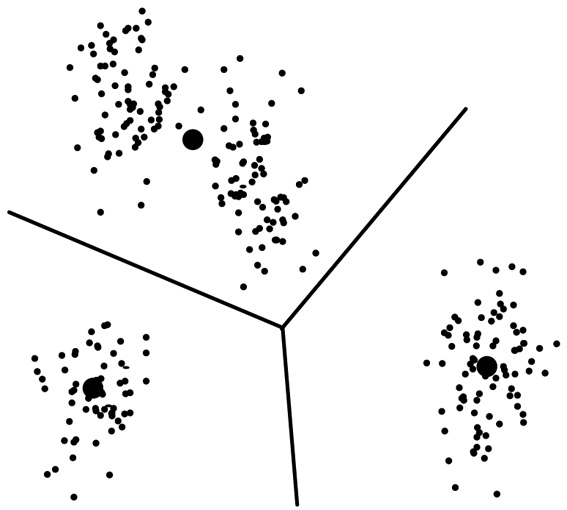
\includegraphics[width=5cm]{images/xmeans1.jpg}}\vspace{1mm}
  \subfloat[Selección punto de partida de K-Means ($k=2$).]{
   \label{f:step2}
    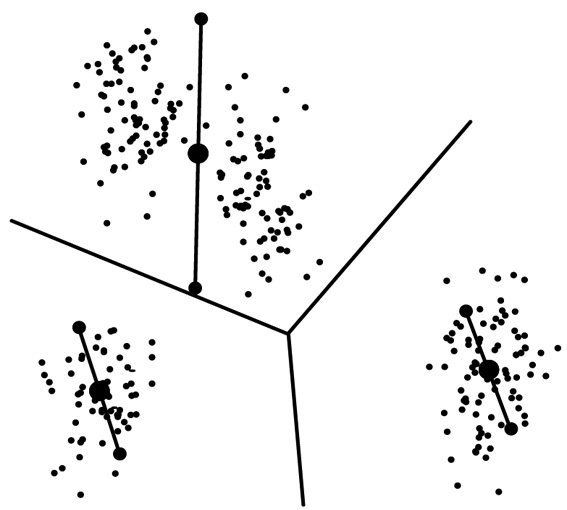
\includegraphics[width=5cm]{images/xmeans2.jpg}}\hspace{1mm}
  \subfloat[Resultado K-Means, evaluación BIC.]{
   \label{f:step3}
    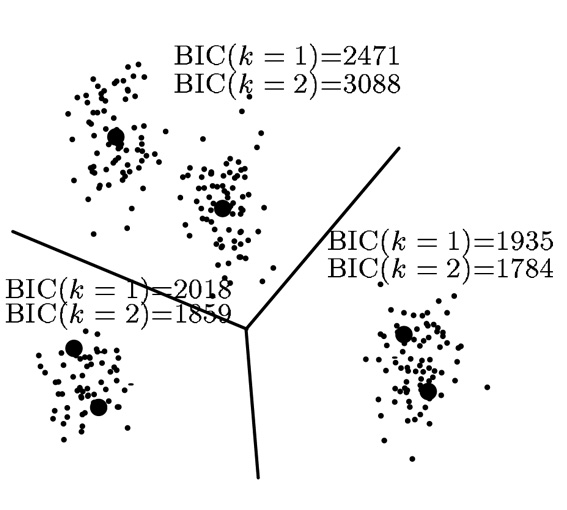
\includegraphics[width=5cm]{images/xmeans3.jpg}}\vspace{1mm}
  \subfloat[Resultado iteración X-Means]{
   \label{f:step4}
    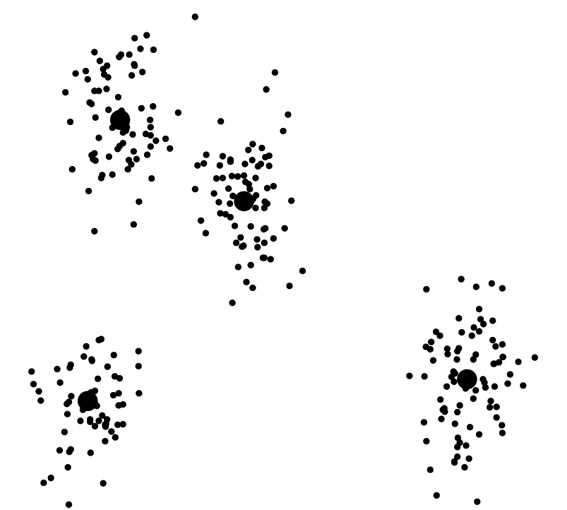
\includegraphics[width=5cm]{images/xmeans4.jpg}}
 \caption{Iteración X-Means.}
 \label{f:xmeans_steps}
\end{figure}

\subsection{Ventajas}

Una de las principales ventajas que posee este algoritmo radica en que es más escalable debido a que con cada iteración se reduce más el número de datos en los cuales K-Means se debe ejecutar, lo que hace que sea más fácil utilizarlo en conjuntos de datos de mayor tamaño. Otra ventaja es que se sabe que con K-Means de pocos clústers es menos probable incurrir en mínimos locales en comparación a uno realizado con muchos clústers. Por lo tanto, el hecho de que X-Means utilice un K-Means con $K=2$ favorece a que no se atasque en mínimos locales.

Además este método permite realizar una visualización del tipo árbol, la que crea una estructura jerárquica de los clústers.